\part{Streszczenie}
Niniejszy dokument zawiera wyniki pomiaru czasu, którego potrzebował mój komputer na wykonanie operacji mnożenia przez 2 na zestawach danych o długościach od 1 do 10e8 elementów. Zawiera także dokumentację kodu programu użytego do wykonania tego badania.

\part{Sprawozdanie}
Obliczenia wykonano na 64-bitowym procesorze AMD Athlon X2. Wykres przedstawia zależność czasu wykonywania operacji od długości ciągu danych. Został wygenerowany za pomocą Gnuplota. Podziałki na obydwu osiach są w skali logarytmicznej. Na wykresie umieszczono także prostą y = (0.7803/10e8)x. Dzięki temu lepiej widać, że jest to zależność mocno zbliżona do liniowej - można na tej podstawie domniemywać, że złożoność obliczeniowa tej operacji jest O(n). Warto zwrócić uwagę na długość wykonywania operacji na jednym elemencie danych - przewyższa on o rząd wielkości czas wykonywania na dziesięciu elementach.
\centerline{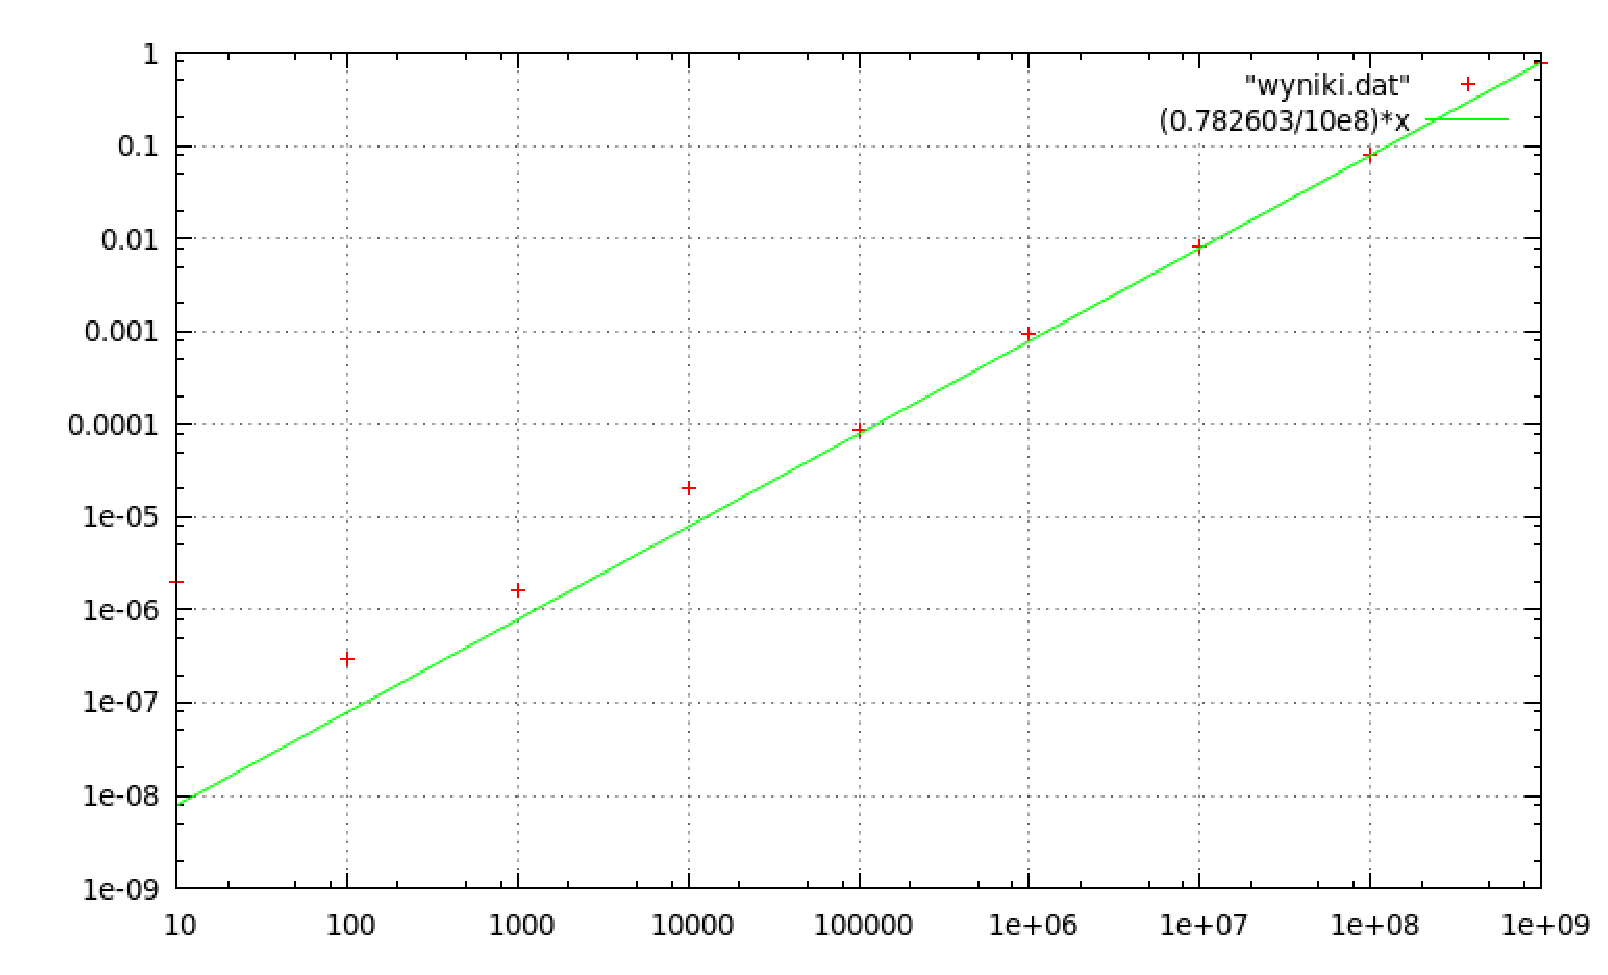
\includegraphics[width=\textwidth,height=\textheight,keepaspectratio]{wykres1.eps}}
